\section{Fabrik Spiel in Unity}\label{sec:factory}
Um zu sehen, welches Potential die Datenorientierte Programmierung in der Spieleentwicklung bietet, wurde eine Spielsimulation sowohl datenorientiert als auch objektorientiert erstellt\footnote{Der Quellcode für die objektorientierte Umsetzung kann zur Reproduktion der Experimente unter \url{https://github.com/dennis12493/FactoryGameSimulationOOP} gefunden werden. Der Quellcode für die datenorientierte Umsetzung findet man unter \url{https://github.com/dennis12493/FactoryGameSimulationDOP}.}. Die Spielesimulation ist eine Art Aufbauspiel, welche mit dem populären Spiel Factorio\footnote{https://www.factorio.com/} verglichen werden kann. Hier wird es jedoch etwas schlichter und einfacher gehalten. Um beide Programmierparadigmen miteinander zu vergleichen, wird eine kleine Fabrik, welche Stahl produziert, in der Spielwelt generiert und vervielfältigt. Dies soll einen Spieler simulieren, der mehrere Fabriken in die Spielwelt platziert. In Abbildung \ref{fig:steel} sieht man wie eine Produktionsstraße für Stahl in dem Spiel aussehen kann.
\begin{figure}[H]
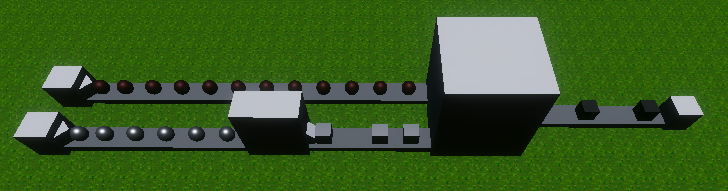
\includegraphics[scale=0.87]{Bilder/Stahl Fabrik.png}
\caption[Eine Stahl Fabrik in der Unity Spielesimulation]{Eine Stahl Fabrik in der Unity Spielesimulation. Links wird Kohle und Eisenerz gefördert. Die Items werden immer von links nach rechts mit Förderbändern zu dem nächsten Kasten weiterbewegt. Das Eisenerz wird zu Eisenbarren geschmolzen (siehe unteres linkes Förderband). In dem großen Kasten wird aus der Kohle und den Eisenbarren Stahl produziert und in dem rechten Kasten verbraucht.}
\label{fig:steel}
\end{figure}
Ganz links befinden sich zwei Kästen. Diese sollen Erzbohrer darstellen, welche Eisenerz (silbern) und Kohle (braun) aus der Erde befördern und rechts auf ein Förderband legen. Die beiden Förderbänder transportieren die Kohle und das Eisenerz nach rechts weiter. Das Eisenerz wird als nächstes in Eisenbarren geschmolzen und ist danach rechteckig. Die Kohle und die Eisenbarren kommen dann gemeinsam in den großen Würfel, wo sie zu Stahl verarbeitet werden. Dieser Stahl wird dann wieder auf ein Förderband gelegt und in dem kleinen Würfel anschließend verbraucht. Die ganze Produktionskette soll einem Videospiel nahekommen, damit es eine möglichst realistische Simulation bietet. Nachfolgend wird gezeigt, wie die Spielsimulation objektorientiert und datenorientiert umgesetzt und gebenchmarkt wird.
\subsection{Objektorientierte Programmierung}
In der Objektorientierten Programmierung mit Unity dreht sich alles um GameObjects. Jedes Objekt in der Szene, egal ob sichtbar oder nicht ist ein GameObject. Diese GameObjects können verschiedene Komponenten haben, welche Eigenschaften definieren, also Daten speichern. Diese Komponenten sind jedoch nicht zu verwechseln mit den \textit{Components} aus dem datenorientierten Ansatz von Unity. Diese Komponenten haben jeweils eine \texttt{Start} und eine \texttt{Update} Methode welche das Verhalten definieren. Die Start Methode wird einmalig vor dem ersten Aufruf der \texttt{Update} Methode ausgeführt. Die \texttt{Update} Methode läuft ein mal pro ausgegebenem Bild. Das Skript für das Item sieht wie folgt aus:
\begin{lstlisting}[style=code, caption={Item Komponente OOP}]
public class Item : MonoBehaviour
{
    private int2 pos;
    //Serialisiertes Feld für den Unity Editor
    [SerializeField] private int itemID;

    void Update()
    {
    	//Gegenstand wird zu der übergebenen Position pos bewegt
        transform.position = Vector3.Lerp(transform.position,
            new Vector3(pos.x, pos.y, -0.5f), Time.deltaTime * 2f);
    }

    public void SetPosition(int2 pos)
    {
        this.pos = pos;
    }
}
\end{lstlisting}
Wie man sieht beinhaltet das MonoBehaviour nicht nur die Daten, sondern auch die Logik. Für ein Item benötigen wir zum einen die Position, wohin sich das Item bewegen soll, zum anderen speichern wir auch eine ID über die wir das Item ganz einfach identifizieren können. Das Attribut \glqq SerializeField\grqq{} zwingt Unity dazu ein editierbares Feld im Editor zu erstellen an dem man die itemID setzen kann.
\begin{figure}[H]
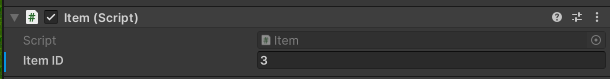
\includegraphics[scale=1]{Bilder/SerializeField.png}
\caption{Ein editierbares Feld in dem Unity Editor. Das Feld wird durch ein public Attribut, oder dem SerializeField Flag erzeugt.}
\label{fig:SerializeField}
\end{figure}
Eine Start Funktion ist in diesem Fall nicht notwendig. Die \texttt{Update} Methode bewegt das Item langsam an die übergebene Position. Time.deltaTime gibt die Zeit in Sekunden von dem letzten Bild bis zu dem momentanen Bild an. Dadurch wird die Bewegung linear.\\
Ein weiterer Teil der Spielesimulation ist die Bewegung der Items über das Förderband. Das Förderband übergibt die Position an das Item und bestimmt daher, in welche Richtung sich das Item bewegen soll:
\begin{lstlisting}[style=code, caption={Förderband Komponente OOP}]
public class BeltPath : MonoBehaviour
{
    private List<ConveyorComponent> beltPath = new ();
    //Referenzen auf die Komponenten des GameObjects werden geholt
    private InputConveyorComponent input 
        = GetComponent<InputConveyorComponent>();
    private OutputConveyorComponent output 
        = GetComponent<OutputConveyorComponent>();
    private float timeToMove = 2f;

    public void Update()
    {
        timeToMove -= Time.deltaTime;
        //Bewegung der Items wird alle 2 Sekunden durchgeführt
        if(timeToMove > 0) return;
        
        var lastBelt = beltPath[^1];
        if (!ReferenceEquals(lastBelt.item, null) && ReferenceEquals(output.GetItem(), null))
        {
            //Gegenstand von dem letzten Förderbandsegment auf den Output legen
            var item = lastBelt.item;
            var itemComponent = item.GetComponent<Item>();
            itemComponent.SetPosition(output.GetPosition());
            output.SetItem(item);
            lastBelt.item = null;
        }
        //Gegenstände von hinten nach vorne um ein Segment verschieben
        for (int i = beltPath.Count-2; i >= 0; i--)
        {
            var thisConveyor = beltPath[i];
            var lastConveyor = beltPath[i + 1];
            if (!ReferenceEquals(thisConveyor.item, null))
            {
                if (ReferenceEquals(lastConveyor.item, null))
                {
                    //Item kann verschoben werden
                    var item = thisConveyor.item;
                    var itemComponent = item.GetComponent<Item>();
                    lastConveyor.item = item;
                    //Position des Items aktualisieren
                    itemComponent.SetPosition(lastConveyor.pos);
                    thisConveyor.item = null;
                }
            }
        }
        var firstConveyor = beltPath[0];
        input.SetOccupied(!ReferenceEquals(firstConveyor.item, null));
        if (!ReferenceEquals(input.GetItem(), null) && ReferenceEquals(firstConveyor.item, null))
        {
            //Item wird von dem Input auf das erste Segment gelegt
            firstConveyor.item = input.GetItem();
            input.RemoveItem();
        }
        //Zeit wird wieder hochgestellt
        timeToMove += 2f;
    }
}
\end{lstlisting}
Für das Förderband wird eine Liste mit vorhandenen Segmenten, der Input, der Output und eine Zeit gespeichert. Die Zeit wird in der Start Methode initialisiert und der Input bzw. Output wird über die Funktion \glqq GetComponent()\grqq{} von dem GameObject geholt. In der \texttt{Update} Funktion wird zunächst nur die timeToMove Variable herunter gezählt. Sollte diese Variable unter Null fallen, werden alle Items von hinten nach vorne ein Segment weiter bewegt sofern dies möglich ist. Ist der Output nicht belegt wird ein vorhandenes Item in den Output gelegt. Items auf den einzelnen Segmenten werden nach weiterbewegt und wenn ein Item im Input liegt wird dies auf das erste Segment weiterbewegt. Immer wenn ein Item weitergegeben wird (egal ob an ein Segment, oder an den Output) wird auch die neue Position an das Item weitergegeben. Durch das bewegen der Items von hinten nach vorne verhindert man, dass sich Items nicht bewegen, obwohl sie es könnten.\\
Auf den Förderbändern sind Items richtige Objekte. In Gebäuden wird lediglich mit \texttt{ItemID's} gearbeitet, da man hier keine sichtbaren Objekte braucht. Um zu sehen, wie Items auf des Förderband gelangen und erstellt werden kann man sich die \texttt{Update} Methode einer Output Komponente eines Gebäudes anschauen:
\begin{lstlisting}[style=code, caption={Create Item OOP}]
void Update()
{
    //Wenn der Output leer ist gibt es nichts zu tun
    if(itemID == -1) return;
    outputGameObject ??= BuildingDictionary.Instance.GetGameObjectAtPosition(pos);
    if (ReferenceEquals(outputGameObject, null) ||
        !outputGameObject.TryGetComponent(out InputConveyorComponent input)) return;
    //Wenn Input des Förderbandes belegt ist wird auch keine
    //Änderung vorgenommen
    if(input.IsOccupied() || !ReferenceEquals(input.GetItem(), null)) return;
    var itemGameObject = Items.INSTANCE.GetItem(itemID);
    //Item wird erstellt
    var item = Instantiate(itemGameObject, new Vector3(pos.x, pos.y, -0.5f), Quaternion.identity);
    item.transform.localScale = new Vector3(0.5f, 0.5f, 0.5f);
    var itemComponent = item.GetComponent<Item>();
    itemComponent.SetPosition(pos);
    var inputConveyorComponent = outputGameObject.GetComponent<InputConveyorComponent>();
    //Input wird das Item zugewiesen
    inputConveyorComponent.SetItem(item);
    Item wird aus dem Output entfernt
    itemID = -1;
    itemCreated = true;
}
\end{lstlisting}
Da man sich im Objektorientierten, ohne weitere Vorkehrungen, immer auf dem \textit{Main Thread} befindet, lassen sich die Items direkt erstellen und dem Input übergeben. Das Zerstören von Items, also der Fall wenn Items von einem Förderband in ein Gebäude übergeben werden, funktioniert sehr ähnlich zu dem Erstellen von Items.
\subsection{Datenorientierte Programmierung}
In der Datenorientierten Programmierung werden statt der GameObjects \textit{Components} und Systeme entworfen. Dabei werden in der Implementierung des Factory Spiels alle Aspekte des \textit{Datenorientierten Technologie-Stack's} von Unity eingesetzt. Es werden die Daten in \textit{Components} gespeichert, welche von Systemen verarbeitet werden. Die Systeme werden, soweit möglich, so umgesetzt, dass der Burst Compiler verwendet werden kann. Zusätzlich werden Jobs erstellt, welche aus Systemen ausgeführt werden.\\
Das Item \textit{Component} des datenorientierten Ansatzes zeigt \hyperref[lstItemComponent]{Listing \ref*{lstItemComponent}}.
\begin{lstlisting}[style=code, caption={[Item \textit{Component} im datenorientierten Ansatz]Item \textit{Component} im datenorientierten Ansatz. Es werden nur die Daten des Items gespeichert. Die Logik des Items befindet sich in einem System.}, label=lstItemComponent]
public struct ItemComponent : IComponentData
{
    public int2 pos;
    public int itemID;
}
\end{lstlisting}
In dem \texttt{ItemComponent} wird die Position und die ID des Items gespeichert. Was direkt auffällt, ist die klare Trennung der Daten von der Logik, welche sich hier in einem System befindet. Die Logik des objektorientierten Items (\hyperref[lstItemKomponente]{Listing \ref*{lstItemKomponente}}) befindet sich im datenorientierten Ansatz in dem \texttt{ItemSystem} in \hyperref[lstItemSystem]{Listing \ref*{lstItemSystem}}.
\begin{lstlisting}[style=code, caption={[Item System im datenorientierten Ansatz.]Item System zum Bewegen von Items im datenorientierten Ansatz. Aus der \texttt{OnUpdate} Methode wird ein Job geschedult, welcher die Items bewegt.}, label=lstItemSystem]
[BurstCompile(CompileSynchronously = true)]
public partial struct ItemSystem : ISystem
{
    [BurstCompile(CompileSynchronously = true)]
    public void OnUpdate(ref SystemState state)
    {
    	//Job erstellen, Zeit übergeben und schedulen
        new ItemMoveJob
        {
            deltaTime = SystemAPI.Time.DeltaTime
        }.ScheduleParallel();
    }

    [BurstCompile(CompileSynchronously = true)]
    public partial struct ItemMoveJob : IJobEntity
    {
        public float deltaTime;
        
        [BurstCompile(CompileSynchronously = true)]
        private void Execute(ref LocalTransform transform,
            in ItemComponent item)
        {
        	//Gegenstand wird zu der übergebenen Position pos bewegt
            transform = transform.WithPosition(
                Vector3.Lerp(transform.Position.xyz,
                    new Vector3(item.pos.x, item.pos.y, -0.5f),
                deltaTime * 2f));
        }
    }
}
\end{lstlisting}
Das \texttt{ItemSystem} ist durch das implementierte Interface \texttt{ISystem} als System defniniert und kann daher die \texttt{OnUpdate} Methode nutzen. Bei dem Item System kommt zusätzlich auch der Burst Compiler und das Job System zum Einsatz. Das Attribut \texttt{BurstCompile} hilft dem Burst Compiler Methoden zu finden, welche mit Burst kompiliert werden sollen. \texttt{CompileSynchronously} dient dem Testen und besagt, dass erst das System durch den Burst Compiler kompiliert werden muss, bevor es zum ersten Mal ausgeführt wird. Andernfalls könnte das System schon laufen, ohne von dem Burst Compiler profitiert zu haben. Die Methode \texttt{OnUpdate} wird ein mal pro Bild aufgerufen (Zeile 5). Sie ist zu vergleichen mit der \texttt{Update} Methode in einem \texttt{MonoBehaviour}. In der \texttt{OnUpdate} Methode wird der \texttt{ItemMoveJob} erstellt (Zeile 8 - 11). Dieser Job funktioniert mit dem \texttt{ItemComponent} und \texttt{LocalTransform} \textit{Component} eines \textit{Entities}. Das \texttt{LocalTransform} \textit{Component} gibt die Position des \textit{Entities} an. Das \texttt{ItemComponent} \textit{Component} ist in \hyperref[lstItemComponent]{Listing \ref{lstItemComponent}} definiert und speichert die Daten des Items. In dem Job wird das \texttt{LocalTransform} \textit{Component} zum Lesen und Schreiben verwendet (erkennbar durch das Keywort \texttt{ref}) und das \texttt{ItemComponent} lediglich zum Lesen (erkennbar durch das Keywort \texttt{in}) (Zeile 20 - 21). Auch hier wird, wie in dem \texttt{MonoBehaviour}, nun die Position des Items mithilfe der \texttt{Lerp} Funktion von \texttt{Vector3} und den Daten im \texttt{ItemComponent} verändert (Zeile 24 - 26). Dieser Job, welcher die tatsächliche Logik für das Item enthält, wird in der \texttt{OnUpdate} Methode parallel gescheduled (Zeile 11). Dies ist hier speziell sehr vorteilhaft, da es sehr viele Items auf dem Spielfeld geben kann. Dadurch werden nicht tausende Items nacheinander bewegt, sondern alle parallel.\\
Die übergebene Position kommt, wie auch in dem objektorientierten Ansatz, von dem Förderband. Auch hier ist die Förderbandlogik in einem Job implementiert. Die Vorgehensweise, dass man die Items von hinten nach vorne ein Förderbandsegment weiterbewegt bleibt jedoch gleich. Ganz anders ist die Funktionsweise, wenn man Items erstellen will. Da man sich mit einem geschedulten Job nicht mehr auf dem \textit{Main Thread} befindet, kann man Items nicht mehr direkt erstellen.
\begin{lstlisting}[style=code, caption={[Erstellung eines Items im datenorientierten Ansatz.]Erstellung eines Items im datenorientierten Ansatz. Zur Erstellung eines Items aus einem Job, wird ein \textit{Entity Command Buffer} verwendet.}]
[BurstCompile(CompileSynchronously = true)]
[UpdateAfter(typeof(ProcessingBuildingSystem))]
public partial struct CreateItemSystem : ISystem {
    //Lookup um Daten eines anderen Entity auszulesen
    private ComponentLookup<InputConveyorComponent> inputLookup;

    [BurstCompile(CompileSynchronously = true)]
    public void OnCreate(ref SystemState state) {
      	//Für die OnUpdate Funktion wird das ItemEntitiesComponent gebraucht
      	//Darin sind alle Items für das Erstellen gespeichert
        state.RequireForUpdate<ItemEntitiesComponent>();
        inputLookup = state.GetComponentLookup<InputConveyorComponent>();
    }
    
    [BurstCompile(CompileSynchronously = true)]
    public void OnUpdate(ref SystemState state) {
        inputLookup.Update(ref state);
        var ecbSingleton = SystemAPI.GetSingleton
            <BeginSimulationEntityCommandBufferSystem.Singleton>();
        //Entity Command Buffer wird erstellt
        var ecb = ecbSingleton.CreateCommandBuffer(state.WorldUnmanaged);
        var itemEntities = SystemAPI.GetSingleton<ItemEntitiesComponent>();
        // Job wird erstellt und gescheduled
        new CreateItemJob {
            inputLookup = inputLookup,
            ecb = ecb,
            itemEntities = itemEntities
        }.Schedule();
        state.CompleteDependency();
    }
}
\end{lstlisting}
Hier sieht man eine Besonderheit des \textit{Entity Component Systems}, der \textit{Entity Command Buffer} (\textit{ECB}). Dadurch, dass strukturelle Änderungen nur auf dem \textit{Main Thread} passieren dürfen, braucht man einen \textit{ECB} um diese Änderungen zu sammeln und an späteren Stelle auf dem \textit{Main Thread} auszuführen. Dafür wird ein \textit{ECB} erstellt (Zeile 21) und dieser dem Job übergeben (Zeile 26). \hyperref[lstCreateItemJob]{Listing \ref{lstCreateItemJob}} zeigt den Job, der diese strukturellen Änderungen vornimmt.
\begin{lstlisting}[style=code, caption={[Job in dem ein \textit{ECB} verwendet wird]Job in dem ein \textit{ECB} verwendet wird. Der \textit{ECB} sammelt die Änderungen aus dem Job und spielt sie nach dem Job wieder ab.}, label=lstCreateItemJob]
[BurstCompile(CompileSynchronously = true)]
[WithNone(typeof(OutputNotFoundTag))]
public partial struct CreateItemJob : IJobEntity {
    public EntityCommandBuffer ecb;
    //Wenn nur von gelesen wird kann ReadOnly verwendet werden
    [ReadOnly] public ComponentLookup<InputConveyorComponent> inputLookup;
    [ReadOnly] public ItemEntitiesComponent itemEntities;

    [BurstCompile(CompileSynchronously = true)]
    private void Execute(ref OutputProcessingBuildingComponent output) {
        //Wenn die Ausgabe leer ist gibt es nichts zu tun
        if(output.itemID == -1) return;
        var itemID = output.itemID;
        var input = inputLookup[output.outputEntity];
        //Wenn die Eingabe des Förderbandes belegt ist wird auch keine
        //Änderung vorgenommen
        if(input.occupied || input.item != Entity.Null) return;
        //Item wird aus der Ausgabe entfernt und mittels ECB
        //wird ein neues Item erstellt 
        output.itemID = -1;
        output.itemCreated = true;
        var itemEntity = itemEntities.GetEntityWithID(itemID);
        var item = ecb.Instantiate(itemEntity);
        //Position und Item Component des Items werden gesetzt
        ecb.SetComponent(item, LocalTransform.FromPositionRotationScale(
            new float3(output.pos.x, output.pos.y, -0.5f),
            quaternion.identity, 0.5f));
        ecb.SetComponent(item,
            new ItemComponent{pos = output.pos, itemID = itemID});
        //Der Eingabe wird das Item zugewiesen
        ecb.SetComponent(output.outputEntity,
            new InputConveyorComponent {
            item = item, pos = input.pos, occupied = true});
    }
}
\end{lstlisting}
Der \textit{ECB} erstellt das Item (Zeile 23) und ändert noch in den \textit{Components} die Position des Items (Zeile 25 - 29). Zusätzlich wird der Eingabe des Förderbandes das erstellte Item zugewiesen (Zeile 31 - 33). Diese Änderungen werden in dem Job aufgenommen und nach dem Job in der richtigen Reihenfolge angewendet.